% Name: Logistic growth
% Description: A logistic curve that levels off at the carrying capacity K, with its inflection point at K/2 and the exponential curve it follows at first.
% Tags: logistic curve, sigmoid, population growth, differential equation

\usepackage{pgfplots}
\pgfplotsset{compat=1.18}

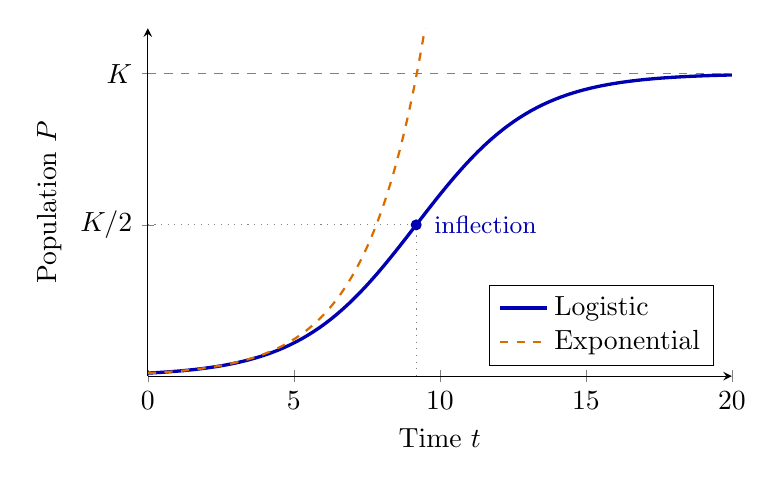
\begin{tikzpicture}
  \begin{axis}[
    width=9cm, height=6cm, axis lines=left, domain=0:20, samples=100,
    xmin=0, xmax=20, ymin=0, ymax=1150, xlabel={Time $t$}, ylabel={Population $P$},
    ytick={500,1000}, yticklabels={$K/2$, $K$}, xtick={0,5,10,15,20},
    legend pos=south east, legend cell align=left,
  ]
    % K = 1000, P(0) = 10, and r = 0.5, so the inflection is at t = ln(99)/0.5 = 9.19.
    \addplot[very thick, blue!70!black] {1000/(1 + 99*exp(-0.5*x))};
    \addplot[thick, dashed, orange!85!black, domain=0:12.2] {10*exp(0.5*x)};
    \draw[gray, dashed] (axis cs:0,1000) -- (axis cs:20,1000);
    \draw[gray, dotted] (axis cs:0,500) -| (axis cs:9.19,0);
    \fill[blue!70!black] (axis cs:9.19,500) circle (2pt) node[right=3pt, font=\small] {inflection};
    \legend{Logistic, Exponential}
  \end{axis}
\end{tikzpicture}
